The semantics of the combination $\pi$-OZ specification S can then be described by the \picalc{} process $S_{OZ\_part_\pi} \mid S_{\pi\_part}$, where $S_{OZ\_part_\pi}$ is the syntactic transformation of \oz{} part into \picalc{} process. For example, the semantics of \refFig{comp_oz_pi_statefull_vm} is $VM\_OZ\_PI \mid VM\_PI$, where $VM\_OZ\_PI$ is as descriped in \refLis{tra_vm_OZ_listing}. Unfortunately, this will not work well, since the parallel operator $|$ only allows the binary synchronization via a channel, not like in $CSP$ where the parallel operator $||$ allows the multiple synchronization via a channel. That will be problematic when we try to combine the $\pi$-OZ specification of an entity S with a $\pi$-OZ specification of another entity R in parallel. To solve this problem we can use \textbf{broadcast channel} or  \textbf{non-atomic reaction} concept as follow:

\subsubsection{Shared channel:}
To allow the multiple synchronization via a channel in \picalc{}, we use concept of the \findex{shared channel}. \cite{ene} introduces the b$\pi$, which is an extension of \picalc{} implementing broadcast communications. Additionaly, the UPPAAL model checker introduces the broadcast channel too \cite{olderog08}. For simplicity, we use the broadcast channel from UPPAAL with a little change. On a shared channel one sender synchronizes with an at least one receiver. Thus, like binary synchronization, a shared channel blocks the sender if there are no receivers. Furthermore, we can send and receive on a shared channel. We extend the transition rules of \picalc{} defined in \refDef{def_pi_trans_system}, with an additional rule:
\begin{figure}[H]
\begin{gather*}
\kalRuleM[if\ x: Shared]{Shared\_Chan\_PAR}{}{P \transs{\out{x}{\vec{y}}} P'}{Q \transs{\inp{x}{\vec{y}}} Q'}{R \transs{\inp{x}{\vec{z}}} R'}{\procpar{\procpar{P}{Q}}{R} \transs{\tau} 
\procpar{P'}{\procpar{\substitue{\vec{y}}{\vec{z}}Q'}{\substitue{\vec{y}}{\vec{z}}R'}}
}
\end{gather*}
\caption{transition rule for shared channel.}
\label{fig_broadcast_channel}
\end{figure}



\refFig{comp_oz_pi_statefull_vm_broadcast} shows the $\pi$-OZ specification of our $VM$ using shared channels.
The combination's process $S_{OZ\_part_\pi} \mid S_{\pi\_part}$ for $VM$ is $VM\_OZ\_PI \mid VM\_PI$. The main advantage of the shared channels in $VM$ is that, if we combine the combination's processes with a third processes $Cus$ representing a customer which issues a signal on the $coffee$ channel, this will enforce both $VM\_OZ\_PI$ and $VM\_PI$ to evolve, since they are listening on coffee, which is shared channel in  $Cus$, $VM\_OZ\_PI$ and $VM\_PI$. The behavior of $VM$ can be seen as the intersection of the behavior of  $VM\_OZ\_PI$ and $VM\_PI$ .i.e. the intersection of the transition graphs .i.e the automates. Unfortunately, our tools do not support the shared channel, thus we will not proceed with this approach.
\begin{figure}[H]
\centering
\begin{class}{VM(id: \integer)}
\ 
\\shared\ chan\ coffee,tea
\ 
\\shared\ chan\ talk:\integer \times \integer
\ \\ \
\\VM\_PI = coffee().VM\_PI + tea().VM\_PI 
\\ \ \qquad \qquad + talk<self,message>.VM\_PI
\\
\begin{state}
self, cv, tv, message: \integer
\ST
0 \leq  cv \leq 3
\\
0 \leq  tv \leq 3
\end{state} 
\\
\begin{init}
self = id
\\cv = 3
\\tv = 3
\\ message= 1
\end{init} 
\\
\begin{op}{coffee}
\Delta (cv)
\ST
cv' = cv - 1
\end{op}
\\
\begin{op}{tea}
\Delta (tv)
\ST
tv' = tv - 1
\end{op}
\\
\begin{op}{talk}
y!: \integer
\\z!: \integer
\ST
y! = message
\\z! = self
\end{op}
\end{class}
\caption{$\pi$-OZ specification of the $VM$ using broadcast channels.}
\label{comp_oz_pi_statefull_vm_broadcast}
\end{figure}



\subsubsection{\findex[non-atomic reaction]{Non-atomic reaction}:} Let us examine the process $Cus \mid VM\_OZ\_PI \mid VM\_PI$ shown in \refFig{binary_reactoin}. When $Cus$ issues a signal on the $coffee$ channel, it is required that $VM\_OZ\_PI$ and $VM\_PI$ receives the signal and evolve together. This is not possible, since the \picalc{} communications are binary, so either $VM\_OZ\_PI$ or $VM\_PI$ will evolve and the other will not. To solve this problem using binary communications we propose to break the channel $coffee$ down into two channels: $ex\_cofee$ and $in\_coffee$ as shown in \refFig{non_atomic_reactoin}. The channel $ex\_cofee$ is for the external, outside $VM$, communication between $Cus$ and $VM\_PI$. The channel $in\_coffee$ is for the internal, inside $VM$, communication between $VM\_PI$ and $VM\_OZ\_PI$. In \refFig{non_atomic_reactoin} the numbered arrows represent the communication flow from $VM\_PI$'s point of view. $VM\_PI$  receives a signal via $ex\_coffee$ and re-sends it via $in\_coffee$. When $VM\_OZ\_PI$ ends its processing it sends a done signal via  $done\_in\_coffee$ to $VM\_PI$ which re-sends the done signal to $Cus$ via $done\_ex\_coffee$. This way the combination's process $S_{OZ\_part_\pi} \mid S_{\pi\_part}$,i.e. $VM\_OZ\_PI \mid VM\_PI$, behaves as a one processes from the view point of its environment .i.e. $Cus$, by breaking down the channel, reproducing the signal, and using the done signal. All that makes the reaction $ordering\ a\ coffee$ a non-atomic reaction. Furthermore, we can notice  that the non-atomic reaction concept is overburdening, since we now have four channels \textit{ex\_coffee, in\_coffee, done\_in\_coffee, done\_ex\_coffee} instead of having one channel for $coffee$.

\refFig{comp_oz_pi_statefull_vm_non_atomic} shows how the $\pi$-OZ specification of $VM$ implements the non-atomic reaction concept. In the interface part it defines the needed channels. For $coffee$ four channels: one external, one internal and two for done signaling. The internal channels $in\_coffee,done\_in\_coffee$ are invisible outside $VM$ Thus we need to extend \oz{} with a new construct $chan\ local$ to define local channels. The local channel is like the $new$ operator in \picalc{},i.e. restriction as follow $VM = new\ in\_coffee,done\_in\_coffee...(VM\_PI\mid VM\_OZ\_PI)$. For $tea$ and $talk$ the same is done like $coffee$. The behavior sequence part $VM\_PI = ex\_coffee().in\_coffee<>.done\_in\_coffee() .... $ reflects exactly the numbered arrows shown in \refFig{non_atomic_reactoin}. 

The $\pi$-OZ specification of $VM$ reads: the combination is ready to participate in an $ex\_cofee$ action issued by the environment. On receiving a signal via $ex\_cofee$, the $\pi$ part will make a transition and issue a signal via $in\_coffee$ enforcing the OZ part to make a transition specified with the operation schema $in\_coffee$. When the OZ part ends its transition it sends a signal via $done\_in\_cofee$ enforcing the $\pi$ part to make a transition, and finally the $\pi$ part issues a done signal via $done\_ex\_cofee$ to the environment declaring that ordering a coffee has done successfully. Notice that the specification has a schema for $in\_coffee$ which represents the conditions on the data, and there no schemes for $ex\_cofee$, $done\_ex\_cofee$ and $done\_in\_cofee$, since they serve for orchestrating.

\refFig{comp_oz_pi_statefull_activeShop_non_atomic} and \refFig{comp_oz_pi_statefull_idleShop_non_atomic} show the $\pi$-OZ specification of $ActiveShop$ and $IdleShop$ respectively, using the non-atomic reaction concept. \refFig{sys_non_atomic_reactoin} shows a big picture of a system consisting of a customer, vending machine and two shops

\begin{figure}[H]%
\centering
\fbox{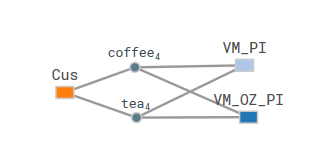
\includegraphics[keepaspectratio,width=0.5\textwidth]{./images/the_compination_pi_oz/binary_reactoin.png}}%
\caption{the process $Cus \mid VM\_OZ\_PI \mid VM\_PI$}
\label{binary_reactoin}%
\end{figure}

\begin{figure}[H]%
\centering
\fbox{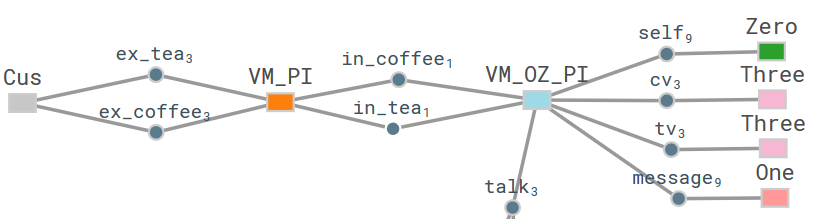
\includegraphics[keepaspectratio,width=0.95\textwidth]{./images/the_compination_pi_oz/non_atomic_reactoin.png}}%
\caption{Action reproducing and non-atomic reaction}
\label{non_atomic_reactoin}%
\end{figure}

\begin{figure}[H]
\centering
\begin{class}{VM(id: \integer)}
\ 
\\chan\ ex\_coffee,in\_coffee,ex\_tea,in\_tea
\ 
\\chan\ talk:\integer \times \integer
\ \\ \
\\VM\_PI = ex\_coffee().in\_coffee<>.VM\_PI 
\\ \ \qquad \qquad + ex\_tea().in\_tea<>.VM\_PI 
\\ \ \qquad \qquad + talk<self,message>.VM\_PI
\\
\begin{state}
self, cv, tv, message: \integer
\ST
0 \leq  cv \leq 3
\\
0 \leq  tv \leq 3
\end{state} 
\\
\begin{init}
self = id
\\cv = 3
\\tv = 3
\\ message= 1
\end{init} 
\\
\begin{op}{in\_coffee}
\Delta (cv)
\ST
cv' = cv - 1
\end{op}
\\
\begin{op}{in\_tea}
\Delta (tv)
\ST
tv' = tv - 1
\end{op}
\\
\begin{op}{talk}
y!: \integer
\\z!: \integer
\ST
y! = message
\\z! = self
\end{op}
\end{class}
\caption{$\pi$-OZ specification of the $VM$ using broadcast channels.}
\label{comp_oz_pi_statefull_vm_broadcast}
\end{figure}

\begin{figure}[H]
\centering
\begin{class}{ActiveShop(id: \integer)}
\ 
\\chan\ ex\_switch: nil | in\_talk
\ 
\\chan\ local\ in\_switch: nil | in\_talk
\ 
\\chan\ ex\_talk:\integer \times \integer
\ 
\\chan\ local\ in\_talk:\integer \times \integer
\ 
\\chan\ done\_ex\_talk
\ 
\\chan\ local\ done\_in\_talk
\ \\ \
\\ActiveShop\_PI = 
\\ \qquad ex\_talk(y, z).\out{in\_talk}{y,z}
\\ \ \qquad \qquad \qquad .done\_in\_talk().\out{done\_ex\_talk}{}.ActiveShop\_PI 
\\ \qquad + \ in\_switch(x).\out{ex\_switch}{x,ex\_talk}.IdleShop\_PI
\\\begin{state}
self, vmId, message: \integer
\\transferableOperation: nil | in\_talk
\end{state} 
\\
\begin{init}
\\self = id
\\transferableOperation = in\_talk
\end{init} 
\\
\begin{op}{in\_switch\_\_\_\_\ then\ IdleShop}
x!: nil | talk
\ST
x! = transferableOperation
\\transferableOperation' = nil
\end{op}
\\
\begin{op}{in\_talk}
\Delta (vmId, message)
\\y?, z?: \integer
\ST
y? = message'
\\z? = vmId'
\end{op}
\end{class}
\caption{$\pi$-OZ specification of the $ActiveShop$ using non-atomic reaction.}
\label{comp_oz_pi_statefull_activeShop_non_atomic}
\end{figure}

\begin{figure}[H]
\centering
\begin{class}{IdleShop(id: \integer)}
\ 
\\chan\ ex\_switch,in\_switch: nil | talk
\ \\ \
\\IdleShop\_PI = 
\\ \qquad  ex\_switch(x,ex\_talk).in\_switch<x>.ActiveShop\_PI
\\
\begin{state}
self, vmId, message: \integer
\\transferableOperation: nil | talk
\end{state} 
\\
\begin{init}
\\self = id
\\transferableOperation = nil
\end{init} 
\\
\begin{op}{in\_switch\_\_\_\_\ then\ ActiveShop}
\Delta (transferableOperation)
\\x?: nil | talk
\ST
x? = transferableOperation'
\end{op}
\end{class}
\caption{$\pi$-OZ specification of the $IdleShop$ using non-atomic reaction.}
\label{comp_oz_pi_statefull_idleShop_non_atomic}
\end{figure}

\begin{figure}[H]%
\centering
\fbox{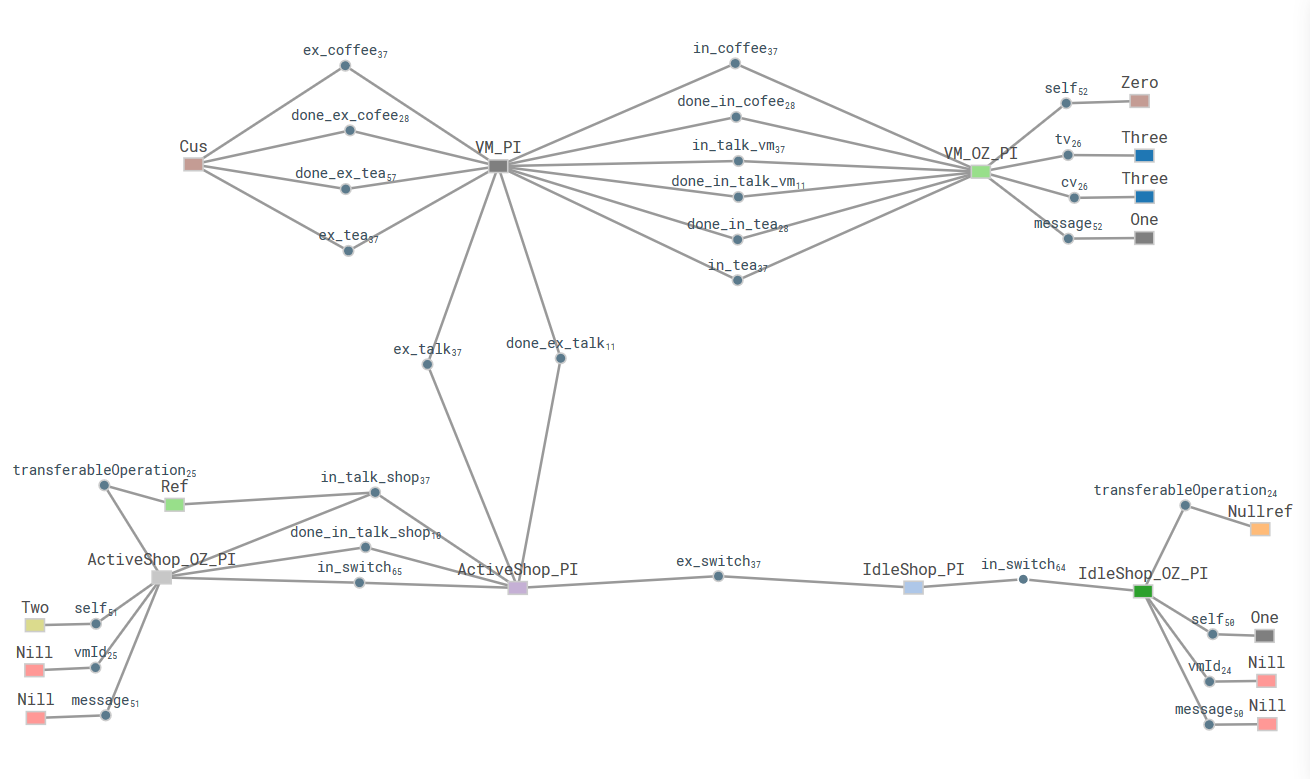
\includegraphics[keepaspectratio,width=0.95\textwidth]{./images/the_compination_pi_oz/sys.png}}%
\caption{system consisting of a customer, vending machine and two shops}
\label{sys_non_atomic_reactoin}%
\end{figure}

Additionally, \refLis{vm_PI_non_atomic} shows the direct implementation of the $\pi$-part of $VM$ specification shown in \refFig{comp_oz_pi_statefull_vm_non_atomic} using ABC code. We can notice that: \\
ex\_coffee.\textquotesingle in\_coffee.done\_in\_cofee.\textquotesingle done\_ex\_cofee.VM\_PI... exactly reflects the $\pi$-part of \refFig{comp_oz_pi_statefull_vm_non_atomic}, where the parameters are removed for clarity.

\lstinputlisting[backgroundcolor=\color{white},caption={ VM ($\pi$-part) in ABC code.},captionpos=b, label={vm_PI_non_atomic}]{listings/vm_PI_non_atomic.abc}

\refLis{vm_OZ_non_atomic} shows the direct implementation of the OZ-part of $VM$ specification shown in \refFig{comp_oz_pi_statefull_vm_non_atomic} using ABC code.

\lstinputlisting[backgroundcolor=\color{white},caption={ VM (OZ-part) in ABC code.},captionpos=b, label={vm_OZ_non_atomic}]{listings/vm_OZ_non_atomic.abc}

\refLis{vm_OZ_and_PI_non_atomic} shows the direct implementation of the $\pi$-part $\mid$ OZ-part of $VM$ specification shown in \refFig{comp_oz_pi_statefull_vm_non_atomic} using ABC code.

\lstinputlisting[backgroundcolor=\color{white},caption={ the combination $\pi$-OZ of VM in ABC code.},captionpos=b, label={vm_OZ_and_PI_non_atomic}]{listings/vm_OZ_and_PI_non_atomic.abc}

\refLis{system_non_atomic} shows a part of the direct implementation of the system consisting of a customer, vending machine, and two shops shown in \refFig{sys_non_atomic_reactoin} using ABC code.
For the full code please see the appendix.

\lstinputlisting[backgroundcolor=\color{white},caption={ the system consisting of: customer, vending machine and two shops in ABC code.},captionpos=b, label={system_non_atomic}]{listings/system_non_atomic.abc}